%Personal information
\newcommand{\autor}{Anuar Nurlybayev, Pawan Bhatla, Rahul Panicker}
\newcommand{\name}{Anuar Nurlybayev, Pawan Bhatla, Rahul Panicker}
\newcommand{\studiengang}{Automation and Robotics}
\newcommand{\matrikelnr}{234194, 235951, 236536}
\newcommand{\titel}{Model Predictive Control of an Inverted Pendulum}
\newcommand{\art}{Project Group}
\newcommand{\jahr}{2023}
\newcommand{\ausgabetag}{21.\,10.~2022}
\newcommand{\abgabetag}{31.\,07.~2023}
\newcommand{\abgabemonat}{July}
\newcommand{\abgabejahr}{2023}
\newcommand{\nummer}{ie3}
\newcommand{\uni}{Technische Universit�t Dortmund}
\newcommand{\urlieee}{http://www.ie3.tu-dortmund.de}
\newcommand{\professor}{Prof.~Dr.-Ing.~Timm~Faulwasser}
\newcommand{\secondexaminor}{Jens P\"uttschneider, M.Sc.}
\newcommand{\betreuer}{Vorname Nachname}
\newcommand{\cobetreuer}{Vorname Nachname}



\documentclass[
   11pt,                	% Schriftgr��e 11pt
   paper=a4,            	% Layout f�r Din A4
   twoside,             	% Layout f�r beidseitigen Druck
   headinclude,         	% Kopfzeile wird Seiten-Layouts mit ber�cksichtigt
   headsepline,         	% horizontale Linie unter Kolumnentitel
   plainheadsepline,   	 	% horizontale Linie auch beim plain-Style
   BCOR12mm,            	% Korrektur f�r die Bindung
   DIV=15,              	% DIV-Wert fuer die Erstellung des Satzspiegels, siehe scrguide
   parskip=half,        	% Absatzabstand statt Absatzeinzug
   toc=bibliography,	 	% Literaturverzeichnis wird ins Inhaltsverzeichnis eingetragen
   numbers=noenddot			% Kapitelnummern immer ohne Punkt
   openany		]    
   {scrbook}			   			% scrbook-Version mind. 2.8j von 2001/07/30  


\usepackage[ansinew]{inputenc}		% erm�glicht direkte Eingabe von Umlauten. Auch m�glich: latin9, latin1, utf8(?)
\usepackage[T1]{fontenc}			% setzt Kodierung des Ausgabezeichensatzes. T1: Zeichensatz mit Umlauten
%\usepackage[ngerman]{babel}			% Silbentrennung gem�� neuer deutscher Rechtschreibung; comment this line out if you write in English
\usepackage[english]{babel}		% comment this line out, if you write in German
\usepackage{amssymb,amsmath}		% Mathematikumgebung
\usepackage{ifthen}					% if-then-Umgebung
\usepackage{graphicx}				% zur besseren Einbindung von Grafiken
\usepackage{xcolor}					% notwendig f�r Farben in der picture-Umgebung (-> TpX, TexCAD etc.)
\usepackage{nomencl}				% automatische Nomenklatur / Abk�rzungsverzeichnis
\usepackage{url}					% erm�glicht die Ausgabe von URLs als anklickbare Links
\usepackage{scrlayer-scrpage}       % Kopf und Fusszeilen-Layout 
\usepackage[printonlyused, withpage]{acronym}
\usepackage[hidelinks]{hyperref}
\usepackage{pdfpages}				% includepdf
\usepackage[style=ieee,backend=bibtex,url=false,doi=false,isbn=false,date=year,citestyle=numeric-comp,maxbibnames=10,minbibnames=10,maxcitenames=10,mincitenames=10]{biblatex}
\usepackage{caption}
\usepackage{float}
\usepackage{subcaption}
\usepackage{wrapfig}
\usepackage{algorithm}
\usepackage{algpseudocode}
\usepackage[algo2e]{algorithm2e}
\usepackage{pgffor}



\KOMAoptions{cleardoublepage=empty}						% Vakantseiten sind leere Seiten (plain = Nummerierung)
\setkomafont{disposition}{\normalcolor\bfseries}		% verwendet die Serifenschrift auch f�r �berschriften


\def\bflabel#1{{{\textsf{#1}}\hfill}}


\newboolean{inGerman}


% Kopf- und Fu�zeile
\pagestyle{scrheadings}
\setlength{\headheight}{1.1\baselineskip}				% Kofzeilenh�he ver�ndern
\ihead[]{\headmark}              						% Kolumnentitel immer oben innen
\ohead[\pagemark]{\pagemark}     						% Seitennummern immer oben aussen
\ofoot[]{}                       						% Seitennummern in der Fusszeile l�schen


% vermeidet einzelne Zeilen oben und unten auf einer Seite
\clubpenalty = 10000
\widowpenalty = 10000 
\displaywidowpenalty = 10000

\bibliography{lit.bib}			% Literaturverzeichnis (Odner/Verzeichnis)

					

%%%%%%%%%%%%%%%%%%%%%%%%%%%%%%%%%%%%%%%%%%%%%%%%%%%%%%%%%%%%%%%%%%%%%%%%%%%%%%%%%%%%%%%%%%%%%%%%%%%%%%%%%%%%%%%%%%%%
%% main document %%%%%%%%%%%%%%%%%%%%%%%%%%%%%%%%%%%%%%%%%%%%%%%%%%%%%%%%%%%%%%%%%%%%%%%%%%%%%%%%%%%%%%%%%%%%%%%%%%%
%%%%%%%%%%%%%%%%%%%%%%%%%%%%%%%%%%%%%%%%%%%%%%%%%%%%%%%%%%%%%%%%%%%%%%%%%%%%%%%%%%%%%%%%%%%%%%%%%%%%%%%%%%%%%%%%%%%%

\begin{document}
%		\setboolean{inGerman}{true} %uncomment this line if the thesis is in English

		\frontmatter
			\thispagestyle{empty}

\begin{titlepage}


\vspace*{4cm}


\begin{center}
\Large
\textbf{\titel}\\
\vspace*{1cm}
\name\\
\vspace*{1cm}
\normalsize
\art\\	
\nummer\\
\abgabemonat~\abgabejahr
\end{center}

\vspace*{4cm}

\ifinGerman
1. Gutachten: \professor\\
2. Gutachten: \secondexaminor
\else
1. Examinor: \professor\\
2. Examinor: \secondexaminor
\fi


\end{titlepage}
			\cleardoubleemptypage			
			%\begin{titlepage}
	
\thispagestyle{empty}

\begin{minipage}[t]{0.99\textwidth}
		\centering
		
\includegraphics[width=0.98\textwidth]{figures/TUlogo.pdf}
\end{minipage}

Project gruppe f�r \autor\\
\textbf{\titel}

\hrule
\vspace{0.2cm}

Die Integration der regenerativen Erzeugungseinheiten in den europ�ischen Kraftwerkspark und damit in das europ�ische Verbundnetz stellt derzeit eine der gr��ten Herausforderungen in der �kologischen Modernisierung der elektrischen Energieversorgung dar. Innerhalb der regenerativen Energiequellen wird derzeit der Windkraft das gr��te Potential zur Ersetzung
gr��erer, konventioneller Erzeugungsbl�cke zugesprochen. Ihre Standorte befinden sich zuk�nftig jedoch dargebotsbedingt zumeist auf hoher See (sogenannte Offshore"=Windparks) und damit weit entfernt von den nationalen �bertragungsnetzen, so dass ihr Netzanschluss h�ufig nur mittels der Hochspannungsgleichstrom�bertragung (HG�) realisiert werden kann.
Aus Netzsicht erscheint daher nicht mehr der rotierende, massebehaftete Generator als Einspeiser, sondern lediglich der leistungselektronische, tr�gheitslose Umrichter. Im Falle der �berwiegenden Einspeisung aus leistungselektronischen Umrichtern bedeutet dies f�r ein Netz, in dem zur Herstellung des Leistungsgleichgewichts eine Frequenzregelung eingesetzt wird, dass die Leistungsf�higkeit und die Grenzen dieses Regelalgorithmus neu bewertet werden m�ssen. In diesem Zusammenhang stellt sich auch die Frage, inwiefern HG�"=Umrichter einen Beitrag zur Bereitstellung von Momentanreserve und zur Prim�rregelung leisten k�nnen.

Folgende Strukturierung der Arbeit wird vorgeschlagen:

\begin{itemize}
	\item Einarbeitung in die Grundlagen der Hochspannungsgleichstrom�bertragung, Leistungs"~/""Frequenzregelung und Simulationsumgebung PowerFactory
	\item Ermittlung des Einflusses leistungselektronischer Einspeisung auf die Momentanreserve und die Leistungsf�higkeit einer Leistungs"~/""Frequenzregelung in einem Drehstromnetz
	\item Entwurf einer Umrichterregelung, die die Beteiligung des Umrichters an der Bereitstellung der Momentanreserve und der Prim�rregelung erm�glicht
	\item Absch�tzung der Leistungsf�higkeit einer solchen Umrichterbeteiligung
	\item Validierung der gefundenen Zusammenh�nge und Ergebnisse an einem Beispielnetz
	\item Dokumentation der durchgef�hrten Arbeiten
\end{itemize}

Im Anschluss an diese Arbeit ist in einem Vortrag �ber die Ergebnisse zu berichten.

\begin{tabbing}
		Tag der Ausgabe:	\hspace{3.5cm} \= \ausgabetag\\
		Tag der Abgabe: 	\> 								\abgabetag\\
		Zust�ndig: 				\> 								\betreuer\\
											\>								\cobetreuer
\end{tabbing}	
	
\end{titlepage}
			%\cleardoubleemptypage			
			%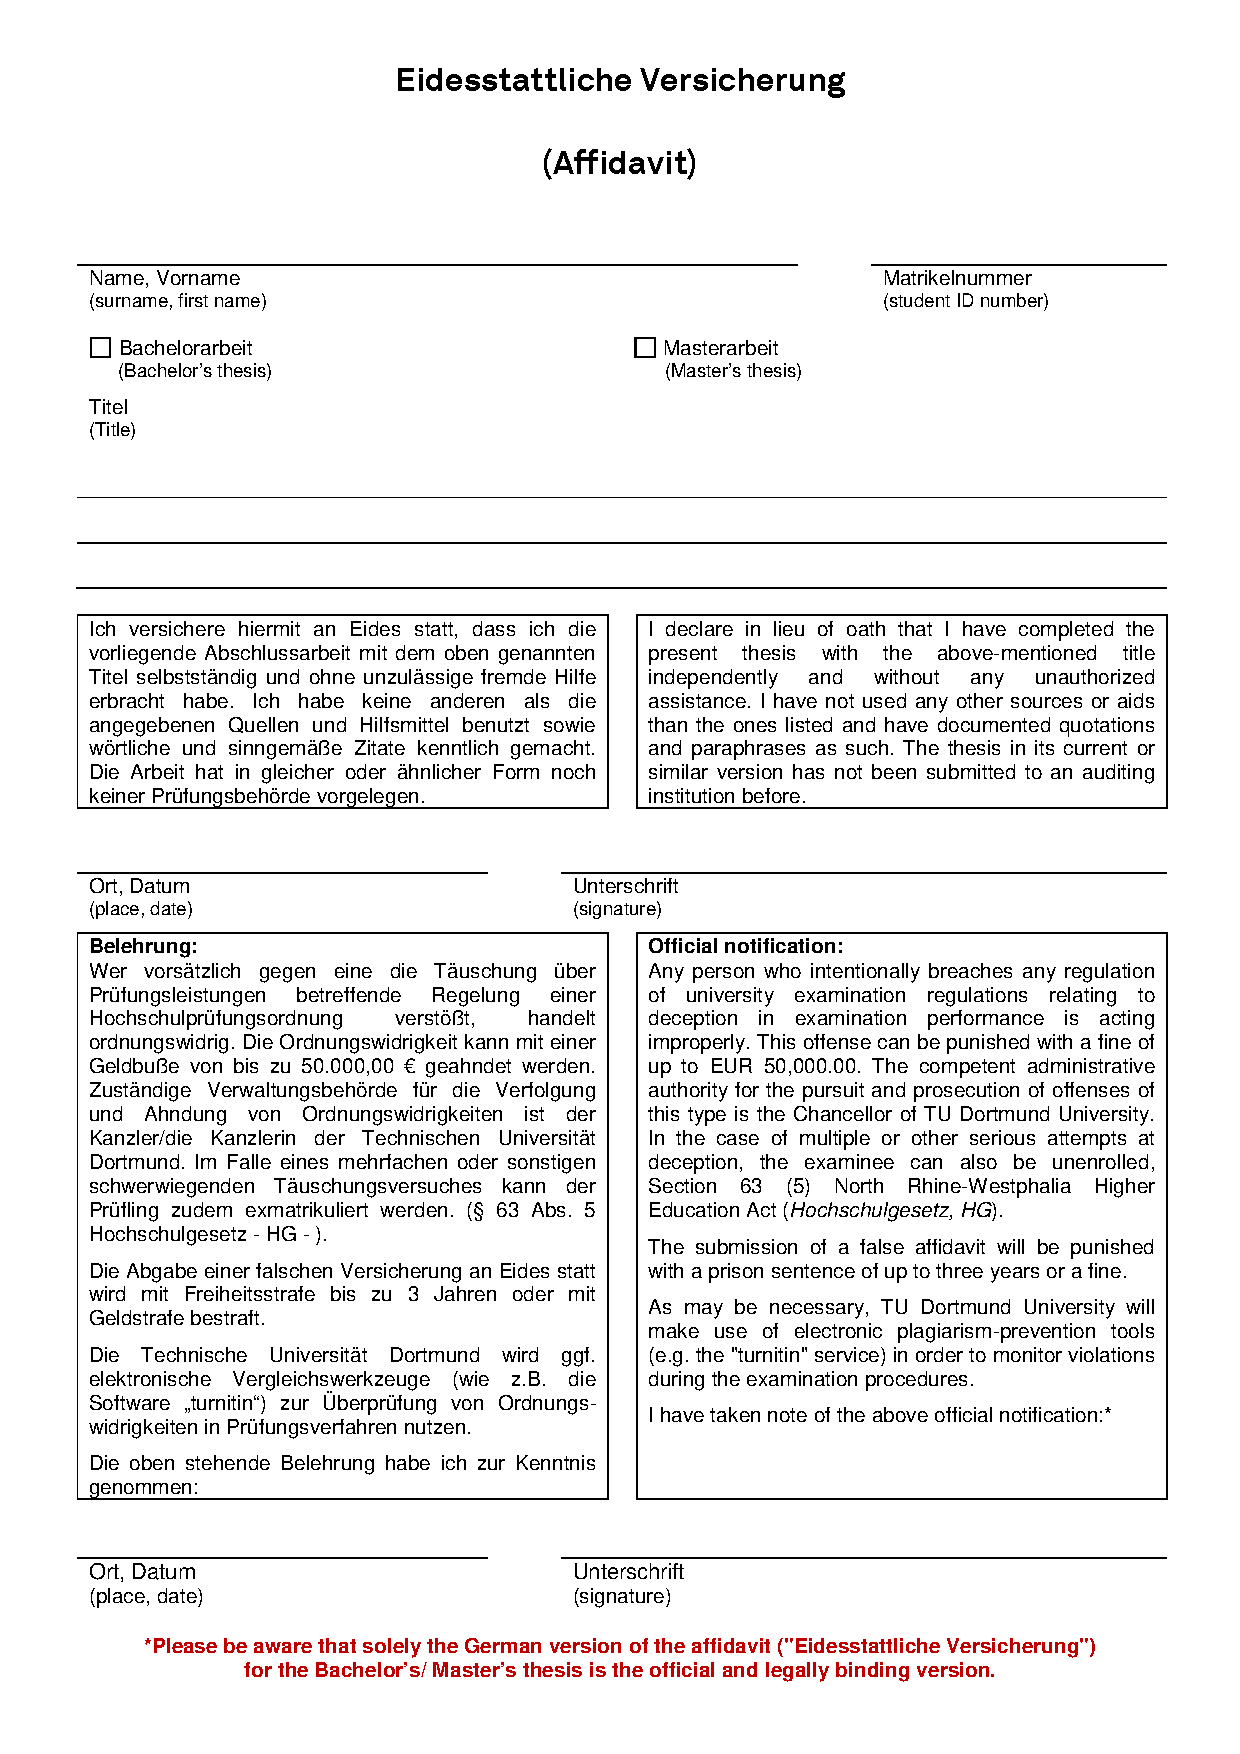
\includepdf{Eidesstattliche_Versicherung.pdf}
			%\cleardoubleemptypage			
			%%%%%%%%%%%%%%%%%%%%%%%%%%%%%%%%%%%%%%%%%%%%%%%%%%%%%%%%%%%%%%%%%%%%%%%%%%%%%%%%%%%%%%%%%%%%%%%%%%%%%%%%%%%%%%%%%%%%
%%%%%%%%%%%%%%%%%%%%%%%%%%%%%%%%%%%%%%%%%%%%%%%%%%%%%%%%%%%%%%%%%%%%%%%%%%%%%%%%%%%%%%%%%%%%%%%%%%%%%%%%%%%%%%%%%%%%
%% Kurzfassung %%%%%%%%%%%%%%%%%%%%%%%%%%%%%%%%%%%%%%%%%%%%%%%%%%%%%%%%%%%%%%%%%%%%%%%%%%%%%%%%%%%%%%%%%%%%%%%%%%%%%
%%%%%%%%%%%%%%%%%%%%%%%%%%%%%%%%%%%%%%%%%%%%%%%%%%%%%%%%%%%%%%%%%%%%%%%%%%%%%%%%%%%%%%%%%%%%%%%%%%%%%%%%%%%%%%%%%%%%
%%%%%%%%%%%%%%%%%%%%%%%%%%%%%%%%%%%%%%%%%%%%%%%%%%%%%%%%%%%%%%%%%%%%%%%%%%%%%%%%%%%%%%%%%%%%%%%%%%%%%%%%%%%%%%%%%%%%

\ifinGerman

\newcommand{\abstracttitle}{Kurzfassung}

\else

\newcommand{\abstracttitle}{Abstract}

\fi

\chapter*{\abstracttitle}
\label{cha:abstract}

\ifinGerman

Hier steht die Kurzfassung.

\section*{\huge Abstract \normalsize}

Hier steht eine englische Version der Kurzfassung.

\else

The stabilization of unstable systems is an important area of research in the field of control systems engineering. Effective control strategies have their origins in human behaviour. The use of predictions of expected behaviour in determining a control strategy is intuitively apparent.

This project explores the development of such a predictive algorithm, namely a model predictive control algorithm for the swing-up and stabilization of an Inverted Pendulum at the upper, unstable equilibrium point.  The inverted pendulum is a popular example for advanced control techniques due to the nature of the system, that is, a highly non-linear system with stabilization around an unstable equilibrium
point.  

The pendulum is mounted on a cart which is connected with a chain to the first encoder, that measures the movement of the cart. The second encoder measures the rotational dynamics of the pendulum.
The developed predictive control algorithm utilizes optimal control to recalculate the input signal to the pendulum and decide the current control output. This recalculation allows the pendulum to reach the desired set point in an optimal fashion. The optimal control problem is built to be solved on a host pc, with Python the programming language of choice. The microcontroller unit on the pendulum, receives the encoder readings and sends it to the host pc. 

Besides the control of the pendulum's angle, it is also necessary to control the angular velocity, linear position and linear velocity of the cart. The algorithm was able to stabilize the pendulum at the central position and in the upright position. 


\fi


			\tableofcontents
			\cleardoubleemptypage
			%%%% acronyms

% \acro{acronym}[short name]{full name}

% \acro{H2O}[$\mathrm{H_2O}$]{water}
% Then \acs{H2O} gets "H2O" and \acl{H2O} prints "water".

%\acrodefplural{ACRONYM}[kuze Pluralform]{lange Pluralform}
%\acrodefplural{BUT}[BUTs]{Blocks Under Test}

\ifinGerman

\chapter*{Abk�rzungsverzeichnis}

\else

\chapter*{Acronyms}
\fi
\label{cha:acronym}

\begin{acronym}[SCOPF]
	\acro{OCP}{Optimal Control Problem}
	\acro{MPC}{Model Predictive Control}
	\acro{LQR}{Linear Quadratic Regulator}
	\acrodefplural{CoG}{Center Of Gravity}
\end{acronym}

			%\cleardoubleemptypage
			\listoffigures
			\cleardoubleemptypage
			%\listoftables
			%\cleardoubleemptypage
			
			
			%Genereller Aufbau einer Abschlussarbeit - Hauptteil
				% 1 Einleitung
				% 2 Theoretische Grundlagen
				% 3 versuchsaufbau/Simulationsmodell
				% 4 Versuchsdurchf�hrung/Simulation und Ergebnisse
				% 5 Diskussion der Simulationsergebnisse
				% 6 Zusammenfassung und Ausblick
				% Anhang
				% Literaturverzeichnis
			
		\mainmatter
			
		 	\chapter{Introduction}
\label{cha:intro}


\section{Motivation}

In the realm of control systems, the inverted pendulum stands as a classic benchmark that fascinates both educators and students. In this project, we delve into the reasons behind the inverted pendulum's popularity as a control benchmark and test an advanced control scheme, namely model predictive control, on said benchmark.

The motivation behind the popular choice of the inverted pendulum as an example for teaching control theory stems from its inherent complexity and non-linearity. Model predictive control, on the other hand, is a relatively young algorithm that combines the areas of optimal control and model-based feedback control to create a controller greater than the sum of its parts. 

Designing and implementing control algorithms for the inverted pendulum gives practical insights into concepts such as feedback control, stability analysis, and system identification. In various domains, such as robotics, aerospace, and automation, systems exhibiting similar dynamics and control challenges can be found.

In summary, the inverted pendulum's excellence as a popular control benchmark lies in its ability to demonstrate core principles of control theory in action, and establish connections to real-world systems. By mastering the control of the inverted pendulum, we acquire valuable skills and insights that are transferable to real-world applications, paving the way for innovation and progress in the field of control systems engineering

\section{Existing Controllers}
The control of inverted pendulum systems has been a topic of extensive research in the field of control systems engineering. Over the years, various controllers have been developed to tackle this task. The controllers implemented in the current iteration of the inverted pendulum involve two major controllers working in tandem, for the two major tasks involved in the control of the inverted pendulum: swing up and stabilization.

\textbf{Energy-Based swing-up controller} addresses a crucial aspect of the inverted pendulum system, the swing-up maneuver. This involves imparting sufficient energy to the pendulum to raise it from the downward hanging position to the upright position. This controller focuses on achieving this energy transfer while simultaneously controlling the system's dynamics. By exploiting the system's potential energy, this controller allows for a smooth and efficient swing-up motion, paving the way for subsequent stabilization using other control techniques.

\textbf{Linear Quadratic Regulator} (LQR) is effectively the simplest optimal controller. A classical control technique widely used for designing optimal control strategies for linear systems. It aims to find a control law that minimizes a quadratic cost function, considering both the system's states and control inputs. The LQR controller for the inverted pendulum system utilizes the system's linearised dynamics and employs state feedback to stabilize the pendulum in an upright position. By formulating the problem as an optimization task, the LQR controller provides an optimal control solution, effectively maintaining stability.

The combination of the LQR controller and the energy-based swing-up controller forms the swing up and stabilization controller for the inverted pendulum system. The energy-based swing-up controller enables the system to transition from an unstable state to a controllable region, while the LQR controller maintains stability and optimal performance once the pendulum is upright. This combined approach allows for a comprehensive control strategy that addresses both the swing-up maneuver and the subsequent stabilization, ensuring the successful control of the inverted pendulum system.

\section{Advanced Controllers}

On further reading one can understand that there are many advanced control schemes that have been devised for the swing up and stabilization of the inverted pendulum system, as alluded to in \cite{Basuki2022,Oishi2018} and one of the frontrunners of these advanced control techniques is the concept of model predictive control. The reason for the popularity of MPC for this particular application are manifold, the primary reason is the ability of MPC to handle non-linear systems along with state and input constraints.
This means that only one controller is necessary for both parts of the pendulum motion as swing up and stabilization can both be done by the same controller.  




% \section{Remarks on the Writing Style}

% Unlike in German, a comma is placed before the last element of a list if that list includes three or more elements in English. Example: popular car brands in Germany are Volkswagen, Audi, and Mercedes.

% Write in the active voice and not in the passive voice. "Albert Einstein developed the special theory of relativity" is preferable to "The special theory of relativtiy was developed by Albert Einstein".

% \section{Remarks on Equations}

% Equations are always part of a sentence. For instance, the circumferene of a circle with radius $r$ is
% \begin{equation}\label{eq:circ}
% U = 2\pi r.
% \end{equation}
% Observe that the period finishing the sentence is part of formula~\eqref{eq:circ} and also observe how labelling the equation in the Latex source code allows to place a reference.

% Use the \texttt{align} command to align equations in multiple rows. Use the \texttt{subequations} command for semantically related equations such as optimization problems with an equation for the objective and equations for the constraints. An example is the Nonlinear Program (NLP)

% \begin{subequations}\label{eq:NLP}
% 	\begin{align}
% 	\min_x \quad &f(x) \\
% 	\text{subject to  } g(x)&=0\\
% 	h(x) &\leq 0.
% 	\end{align}
% \end{subequations}

% Physical units are written in solid font and not in italic font. 
% There should be a semi-space in between the number and the unit, as in $1\,$V.
% The~\texttt{SI} latex package may help you.


% \section{Remarks on Figures}

% Having a list of figures at the beginning of your thesis is benefitial, but not mandatory.

% Every figure must have a caption which describes the content. Ideally, the key message which is conveyed by a figure is summarized in one sentence at the end of the caption.

% Every figure must be referenced in the text.

% Graphs and plots must be displayed as vector graphics. Popular options for this are to include \texttt{.eps} files generated with Matlab, Python, and Julia or \texttt{tikz} pictures. If you use \texttt{tikz} and Matlab, then the \texttt{matlab2tikz} package can hlep you.

% Text within a figure should be sufficiently large to be easily readable. 

% If a figure is taken from another source, then the reference must be cited wtihin the caption.


% \section{Remarks on Tables}

% Having a list of tables at the beginning of your thesis is benefitial, but not mandatory.

% All tables need a caption and must be referenced in the text.

% Do not draw vertical lines in tables to separate columns.

% \section{Remarks on Citations}
% It is preferable to place citations at the end of a sentence. For instance, the design of stabilizing terminal ingredients in optimal control problems is discussed in~\cite{Chen1998}. 

% Imagine the following situation: you read in source A that source B proved a result you wish to use. It would be plagiarism to simply cite source A for this result! Instead you have to find source B, find the result in source B, and then cite source B for the result. If you cannot find source B, then you cite~"\cite{B} according to~\cite{A}". But you should try really hard to find source B.

% Give accurate citations, especially for textbooks or large documents. That is, you should either refer to a specific equation, theorem, figure, or page in a source. For instance, the two norm of a matrix is defined as the largest singular eigenvalue~\cite[p. 88]{Hespanha2018}.



% Helpful resources:
% \begin{itemize}
% 	\item Good scientific practice at TU Dortmund University: \url{https://www.tu-dortmund.de/en/research/research-ethics/good-scientific-practice/}
% 	\item Course on writing in the sciences by Kristin Sainani, Stanford~\url{https://www.youtube.com/watch?v=HxSu-FQ0yl40}
% 	\item Ten rules for mathematical writing by Dimitri Bertsekas~\url{https://www.mit.edu/~dimitrib/Ten_Rules.pdf}
% \end{itemize}

% \chapter{Latex}

% \section{Labels and References}

% Latex allows you to place references to chapters, sections, subsections, equations, figures, tables, and further environments via the \texttt{ref} command.
% It is convenient to use \texttt{eqref} to refer to equations, because \texttt{eqref} automatically adds the required parentheses.
% A good strategy is to give meaningful labels to environments. For instance, \texttt{eq:NLP} is a fitting label for NLP~\eqref{eq:NLP}.
% Popular prefixes are
% \begin{itemize}
% 	\item \texttt{eq} for equations
% 	\item \texttt{fig} for figures
% 	\item \texttt{tab} for tables
% 	\item \texttt{ch} for chapters
% 	\item \texttt{sec} for sections
% 	\item \texttt{thm} for theorems
% \end{itemize} and many more.



		 	%include further chapters here
		 	\chapter{Basics} \label{Chapter 2}
\label{chap:first chapter}

The aim of this project is to study and devise an advanced control method, in this case model predictive control (MPC), for a highly non-linear system with an unstable equilibrium, in this case an inverted pendulum.
As the name suggests, model predictive control involves the mathematical model of the system. By solving an optimization problem using states that are fed back to the this model, one can predict the optimal state trajectory for the next $\mathnormal{N}$ time steps. This $\mathnormal{N}$ is called the prediction horizon of the controller and is an important parameter that can be tuned for better performance.

In this chapter we will look at the mathematical modelling of this system as well some basic MPC theory that enables one to design a stable and optimal controller. 

\section{Inverted pendulum}
The inverted pendulum or the "cart-pole" system, as mentioned before is a standard test case for new control strategies. For MPC it is first important to model this system mathematically, the following section gives an brief overview of the real system followed by the mathematical modelling of this system.

\subsection{Physical System}

The outer construction of the pendulum, as shown in Figure \ref{fig: Outer covering}, consists of extruded aluminium and custom-designed elements made of PET-G material. The internal components, shown in Figure \ref{fig: Internal components} are also custom-designed and made of either PET-G or PLA+ \cite{PendulumManual}.

The internal components consist of the following:
\begin{itemize}
	\item Pendulum connector : Connects the pendulum arm to the cart.
	\item Rotary encoder :To measure the angle of rotation of the pendulum arm.
	\item Cart rails : For cart movement.
	\item Motor : A stepper motor which moves the cart.
	\item Motor driver : Used to control the stepper motor. 
	\item MCU : The ESP32 microcontroller unit responsible for generating the PWM signal for the motor.
	\item Limit switches : 2 limit switches at either side of the cart mark the limits of the cart.
\end{itemize}


\begin{figure}[H]
	\centering
	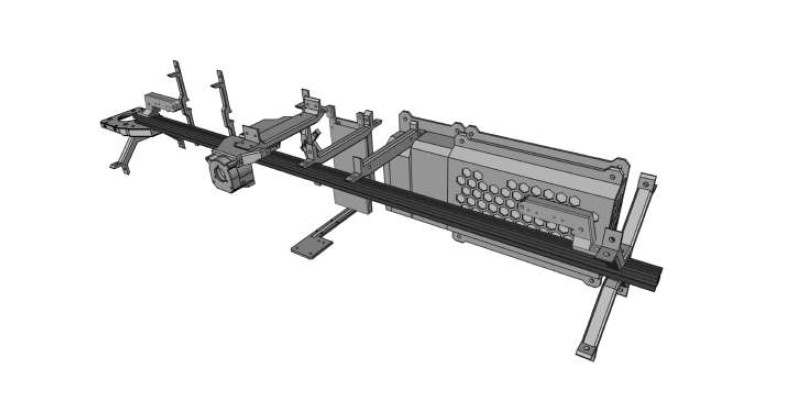
\includegraphics[width=0.75\textwidth]{"src/Images/Pendulum_inner.jpg"}
	\caption{internal components \cite{PendulumManual}.}
	\label{fig: Internal components}
\end{figure}

\begin{figure}[h!]
	\centering
	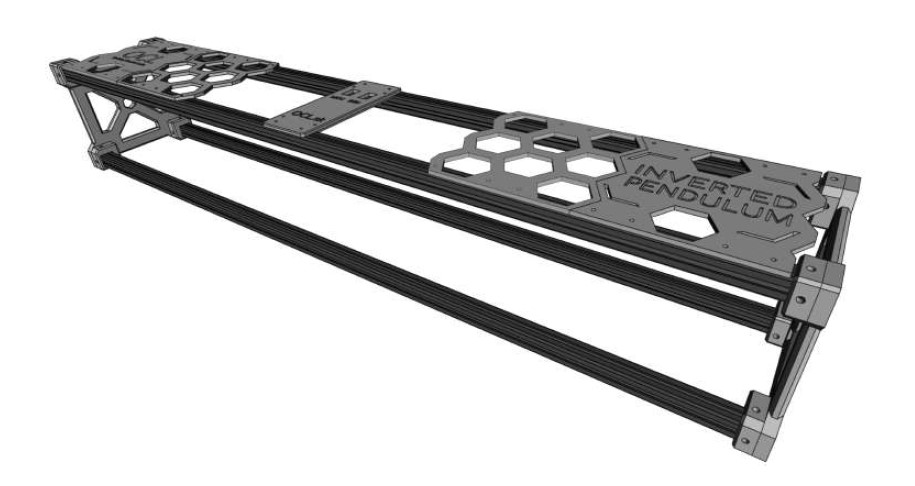
\includegraphics[width=0.75\textwidth]{"src/Images/Pendulum_outer.jpg"}
	\caption{outer covering \cite{PendulumManual}.}
	\label{fig: Outer covering}		
\end{figure}


\begin{figure}[H]
	\centering
	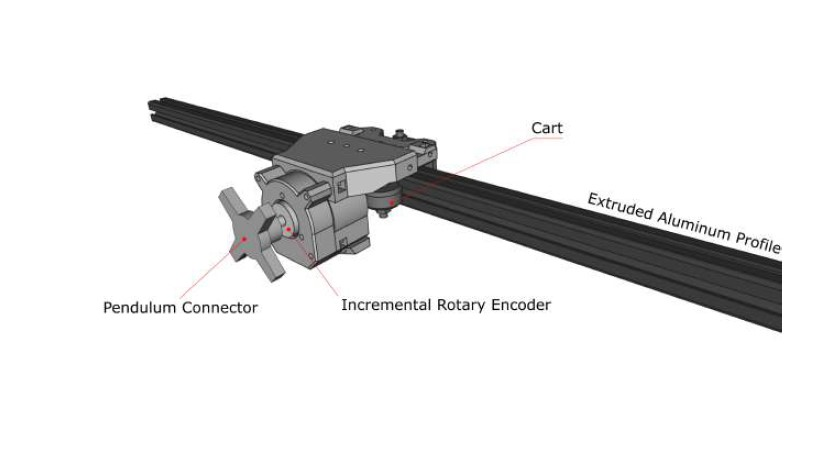
\includegraphics[width=0.75\textwidth]{"src/Images/Pendulum_cart.jpg"}
	\caption{pendulum cart and rotary encoder \cite{PendulumManual}.}
	\label{fig:Pendulum Cart}
\end{figure}  

\begin{figure}[H]
	\centering
	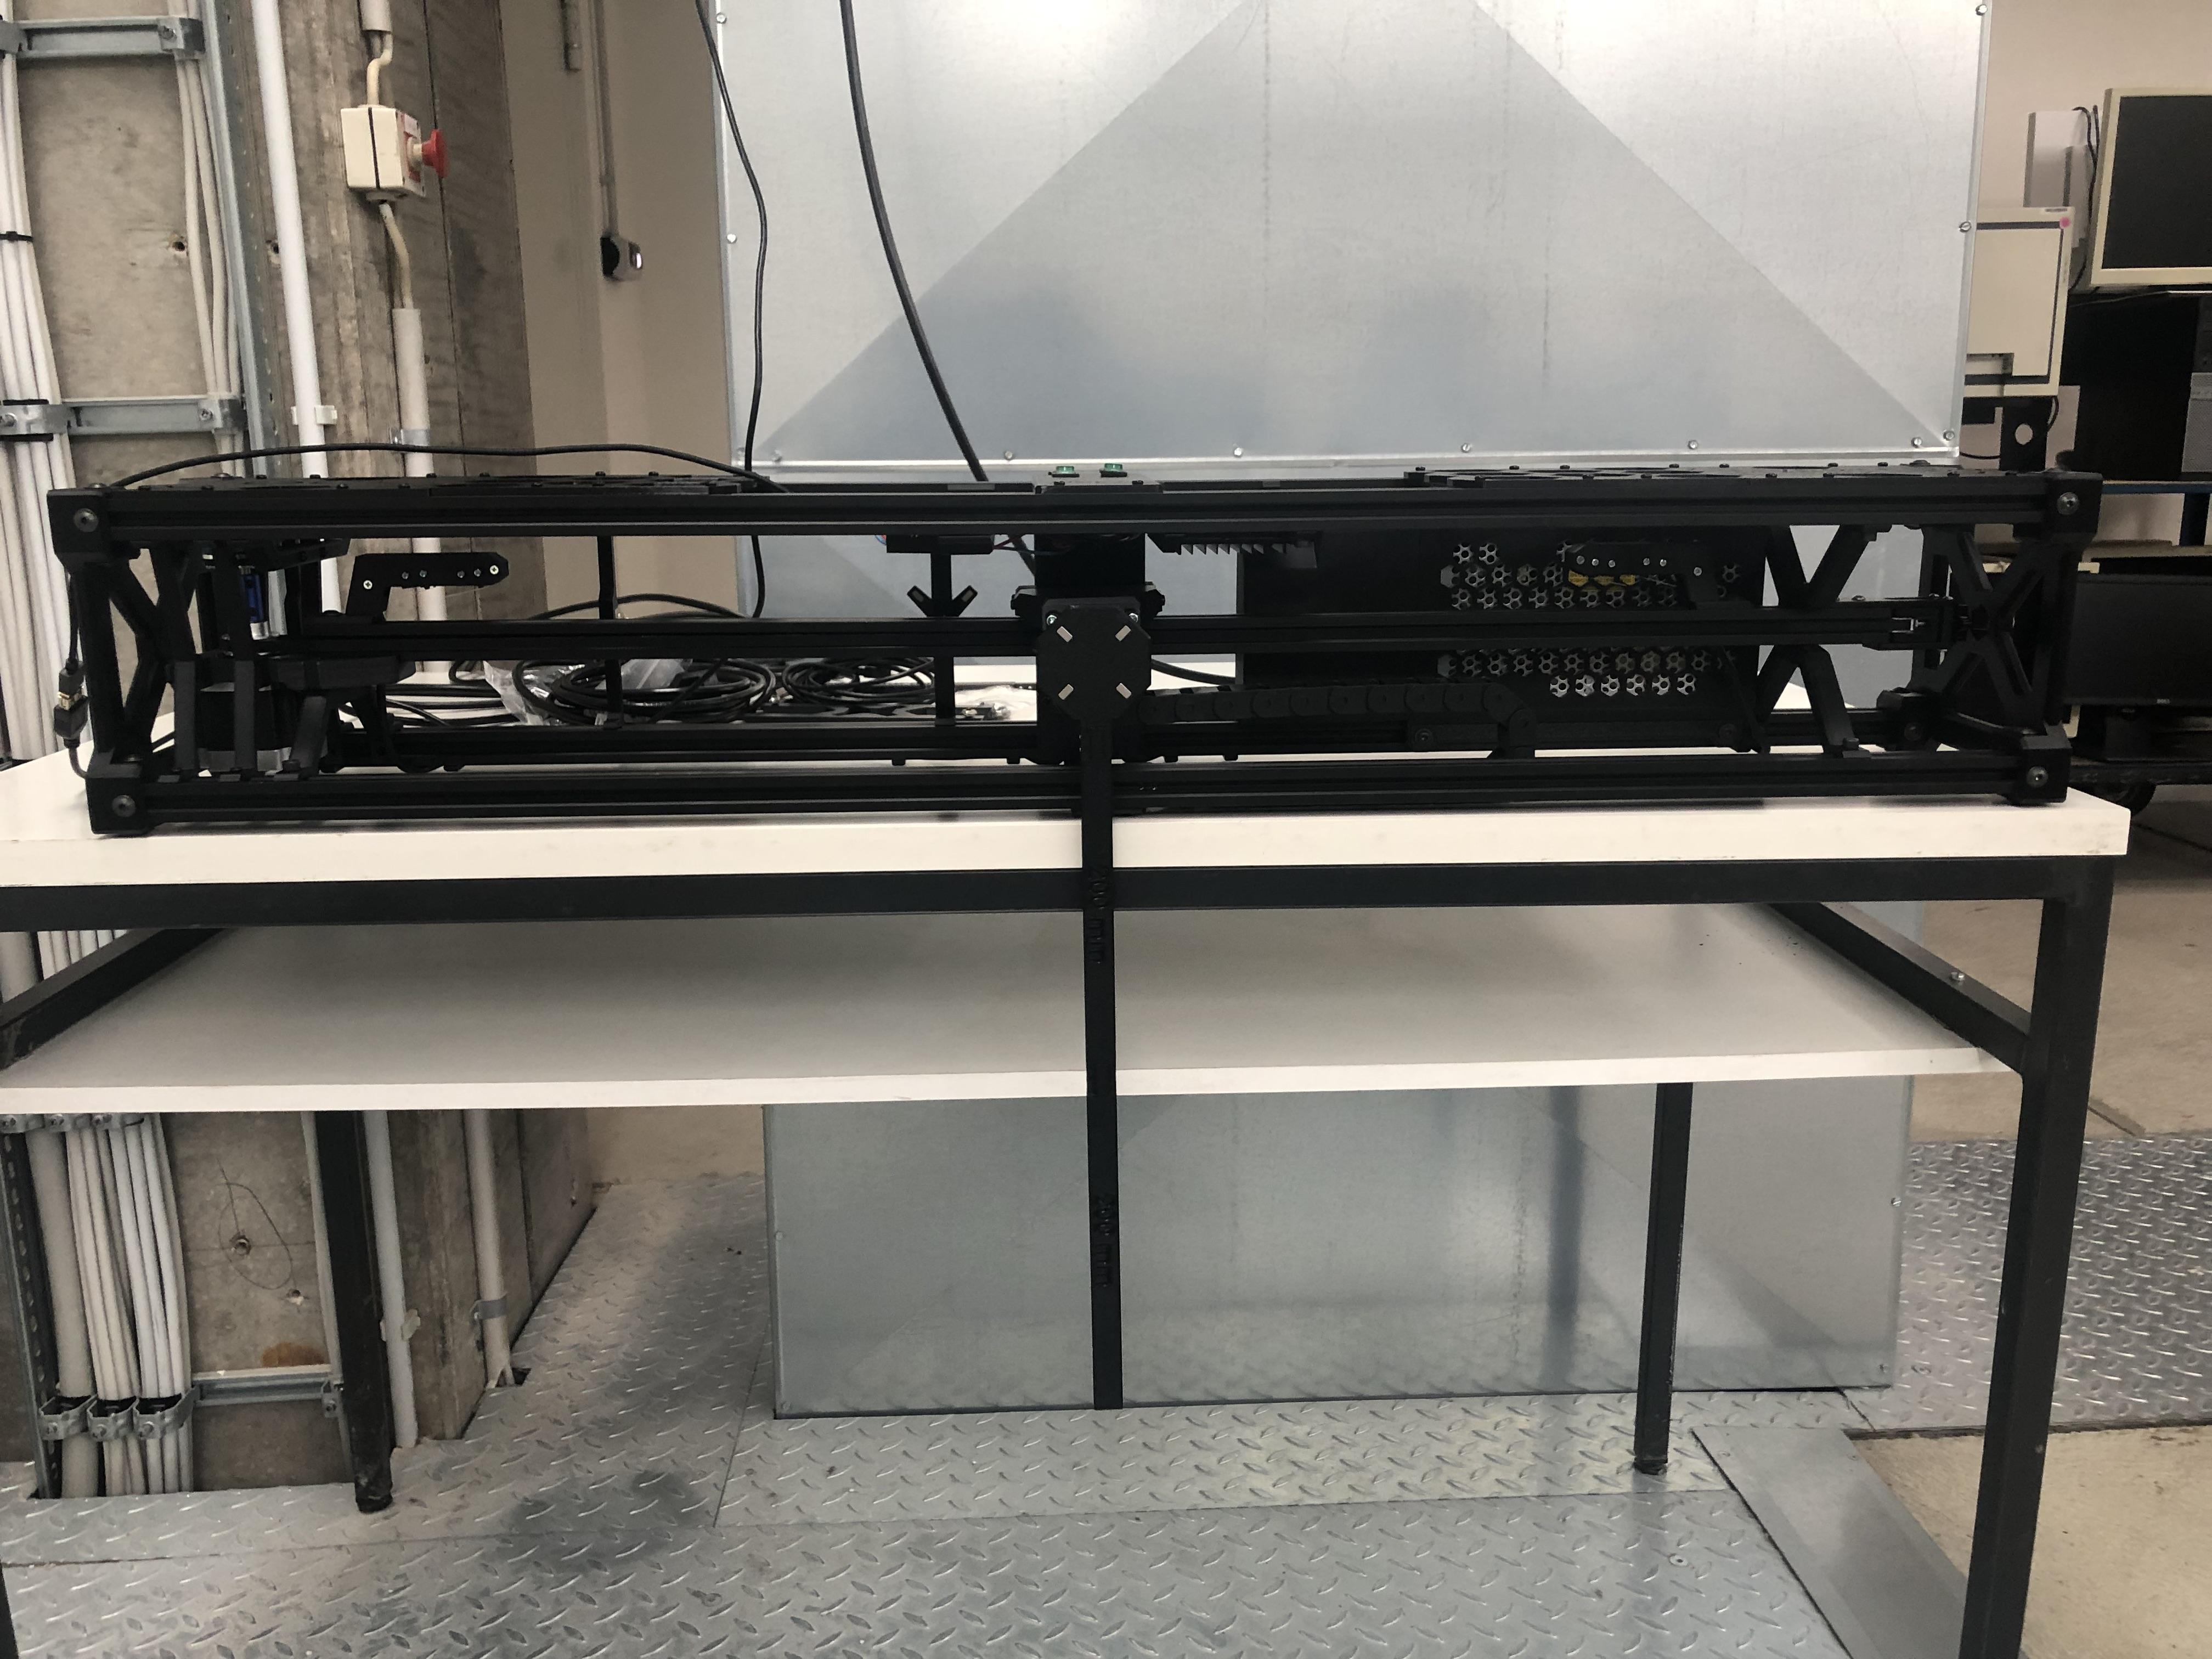
\includegraphics[width=0.75\textwidth]{"src/Images/Real_pendulum1.jpg"}
	\caption{inverted pendulum : front view}
	\label{fig:Real Pendulum}
\end{figure}  


\begin{figure}[h!]
	\begin{subfigure}{0.5\textwidth}
		\centering
		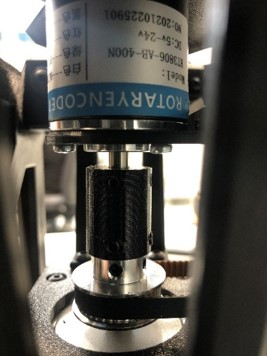
\includegraphics[width=0.6\textwidth]{"src/Images/Motor.jpg"}
		\subcaption{motor and encoder.}
		\label{fig:Motor}
	\end{subfigure}
	\hfill
	\begin{subfigure}{0.7\textwidth}
		\centering
		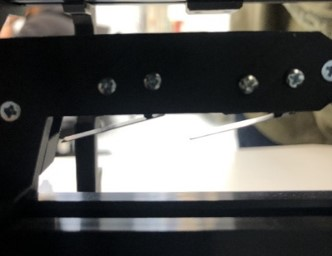
\includegraphics[width=0.6\textwidth]{"src/Images/Limit_Switch.jpg"}
		\subcaption{limit switch.}
		\label{fig:Limit Switch}
	\end{subfigure}
	\caption{pendulum components: motor and limit Switch.}
	\label{fig:Components of the Pendulum : Motor and Limit Switch}
\end{figure}


\begin{figure}[h!]
	
	\begin{subfigure}{0.45\textwidth}	
		\includegraphics[width=\textwidth,scale=0.75]{"src/Images/Real_pendulum3.jpg"}
		\subcaption{ESP32 microcontroller}
		\label{fig:ESP32 Microcontroller}
	\end{subfigure}
	\hfill
	\begin{subfigure}{0.45\textwidth}
		\centering
		\includegraphics[width=\textwidth,scale=0.75]{"src/Images/Real_pendulum4.jpg"}
		\subcaption{motor driver}
		\label{fig:Motor Driver}
	\end{subfigure}
	\caption{pendulum components: microcontroller and driver}
	\label{fig:Components of the Pendulum: Driver and ESP}
\end{figure}  

The motor is controlled using a motor driver and an ESP32 microcontroller, shown in Figure \ref{fig:Components of the Pendulum: Driver and ESP}, that produces Pulse Width Modulated (PWM) signals to control the step angle to produce desired velocities. Since the input chosen was the cart acceleration, we have to first convert this to the cart velocity at current time. This can be done using the relation,  $$v_{cart} = u\cdot dt + v_0 $$ 
where $u$ is the cart acceleration, dt is the sampling time of the pendulum and $v_0$ is the velocity at the previous time step. This is then converted to the frequency of the PWM signal using the relation
$$f_{pwm} = v_{cart}\cdot20,000$$
This is explained in more detail in later chapters. 

\subsection{Mathematical Model} 

We first start by defining a few variables and what they represent in our inverted pendulum system : 	
\begin{itemize}
	\item Cart position: $x(t)$
	\item Pendulum centre of gravity x-Position: $x_s(t)$
	\item Pendulum centre of gravity y-Position: $y_s(t)$
	\item Pendulum angle measured from the top equilibrium: $\theta(t)$
	\item Pendulum length: $\ell$
	\item Pendulum mass: $m$
	\item Pendulum moment of inertia: $J = m\ell^2 / 12$
	\item Angular friction coefficient: $b$
	\item Contact forces between pendulum and cart: $F_x(t), F_y(t)$
	\item Gravity constant: $g$
\end{itemize}

\begin{figure}[htbp]
	\centering
	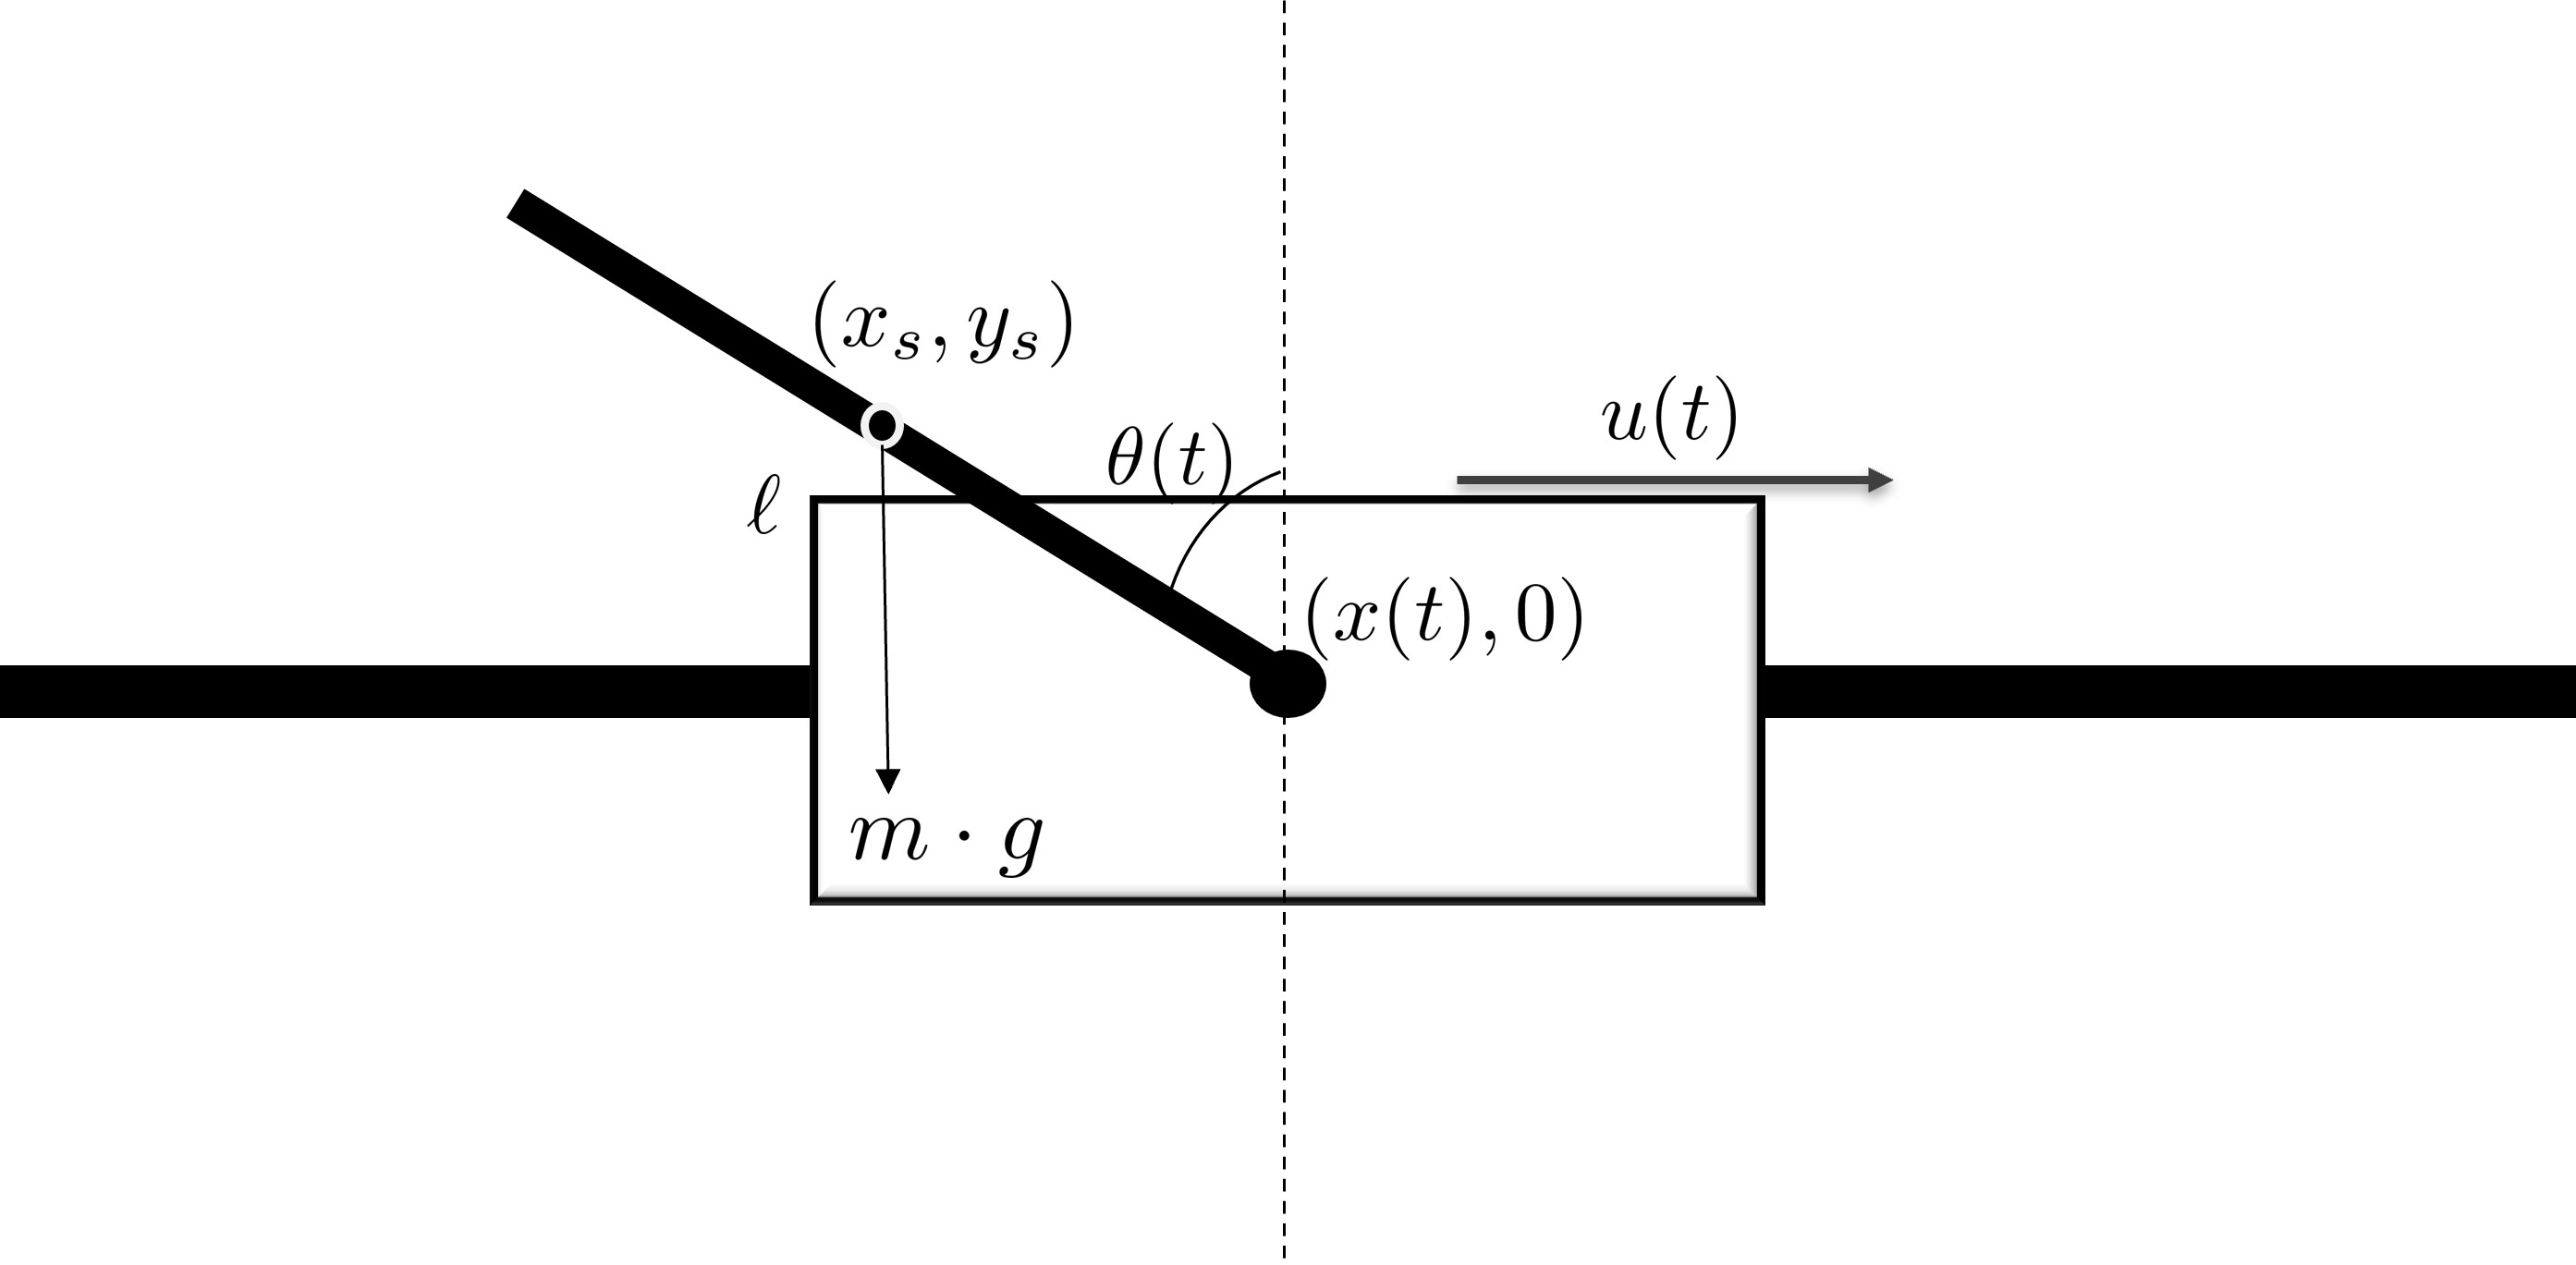
\includegraphics[width=0.5\textwidth]{"src/Images/pendulum1.jpg"}   
	\caption{pendulum schematic}
	\label{fig:Pendulum schematic}
\end{figure}


We then define the coordinates,linear velocity and acceleration of the centre of gravity of the pendulum arm as $(x_s,y_s)$, $(\dot{x}_s, \dot{y}_s)$ and $(\ddot{x}_s,\ddot{y}_s)$ respectively. These can then be calculated as follows:


\begin{align*}
x_s &= x - \frac{\ell}{2} \sin(\theta)\\
\dot{x}_s &= \dot{x} - \frac{\ell}{2}\dot{\theta}\cos(\theta)\\
\ddot{x}_s &= \ddot{x} - \frac{\ell}{2}\ddot{\theta}\cos(\theta) + \frac{\ell}{2}\dot{\theta}^2\sin(\theta)\\
y_s &= \frac{\ell}{2}\cos(\theta)\\
\dot{y}_s &= -\frac{\ell}{2}\dot{\theta}\sin(\theta)\\
\ddot{y}_s &= -\frac{\ell}{2}\ddot{\theta}\sin(\theta)- \frac{\ell}{2}\dot{\theta}^2\cos{\theta}
\end{align*}



In first principle modelling one uses basic physical conservation laws to model the system, in chemical reactors for example, one can use molar balance equations. In this case we use force balance equations.

So applying force balance in x-direction of the pendulum we get:
\begin{equation}\label{eq:xbalance}
m \ddot{x}_s = F_x
\end{equation}

Similarly, applying force balance in y-direction of the pendulum, we get:
\begin{equation}\label{eq:ybalance}
m \ddot{y}_s = F_y - mg
\end{equation}

Another possible quantity that can be balanced is torque, so applying torque balance to the pendulum's centre of gravity (CoG), we obtain:
\begin{equation}\label{eq:torquebalance}
J\ddot{\theta} = F_x \frac{\ell}{2}\cos(\theta) + F_y \frac{\ell}{2}\sin(\theta) - b\dot{\theta}
\end{equation}

Plugging~\eqref{eq:xbalance} and~\eqref{eq:ybalance} into~\eqref{eq:torquebalance} to obtain

\begin{equation}\label{eq: 2.4}
\left(J + m\frac{\ell^2}{4} \right) \ddot{\theta} = m \ddot{x} \frac{\ell}{2}\cos(\theta) + mg \frac{\ell}{2}\sin(\theta) - b\dot{\theta}
\end{equation}
Since $J = m\ell^2 / 12$ we get $(J + m\ell^2/4) = m\ell^2/3$. This results in a reformulated equation which reads:
\begin{equation}
\ddot{\theta} = \frac{3 \cos(\theta)}{2 \ell} \ddot{x} + \frac{3 \sin(\theta)}{2\ell} g - \frac{3b}{m\ell^2} \dot{\theta}
\end{equation}

\begin{equation}
\begin{aligned}
\ddot{\theta} &= \frac{3g}{2\ell} \sin(\theta)    -\frac{3b}{m\ell^2} \dot{\theta}              + \frac{3}{2\ell} \cos(\theta)u\\
\ddot{x} &= u 
\end{aligned}
\end{equation}

We can also redefine the friction coefficient $b'=\frac{3b}{m\ell^2}$, with this we get

\begin{equation}
\begin{aligned}
\ddot{\theta} &= \frac{3g}{2\ell} \sin(\theta)    -b' \dot{\theta}              + \frac{3}{2\ell} \cos(\theta)u\\
\ddot{x} &= u. 
\end{aligned}
\end{equation}

\vspace{0.5cm}

from the above derivation of the system model, one can decide on the states, inputs and outputs of the inverted pendulum model as follows : 

\begin{itemize}
	\item States: 
	\begin{itemize}
		\item $x_1(t) \doteq \theta(t)$  - angular displacement of pendulum
		\item $x_2(t) \doteq \dot{\theta}(t)$ - angular velocity of the pendulum
		\item $x_3(t) \doteq x(t)$    - linear displacement of the cart
		\item $x_4(t) \doteq \dot{x}(t)$ - linear velocity of the cart
	\end{itemize}
	\item Input:
	\begin{itemize}
		\item $u(t) \doteq \ddot{x}(t)$ i.e. input = cart acceleration
	\end{itemize}
	\item Measured quantities: 
	\begin{itemize}
		\item $x_1(t)$ from pendulum encoder
		\item $x_3(t)$ from cart encoder
	\end{itemize}
\end{itemize}

And so the full dynamic equation of the inverted pendulum can be written as 

\begin{equation}
\begin{bmatrix}
\dot{x}_1 \\
\dot{x}_2 \\
\dot{x}_3 \\
\dot{x}_4
\end{bmatrix} = \begin{bmatrix}
x_2\\
\frac{3g}{2\ell} \sin(x_1)    -\frac{3b}{m\ell^2}x_2              + \frac{3}{2\ell} \cos(x_1)u \\
x_3 \\
u
\end{bmatrix}
\end{equation}



\section{Model Predictive Control}

As mentioned before, model predictive control is a very popular strategy among other advanced control methods. There are many reasons for its popularity, some being that it is able to consider the entire non-linear system without any linearising approximations and it is also very adept at handling constraints. 



Model predictive control is intrinsically linked with the concept of optimal control as MPC involves the solution of an open loop optimal control problem (OCP) at every time step. In the simple MPC scheme shown in Figure \ref{fig:MPC Schematic}, the optimal control inputs for the next $p$ steps are calculated and the very first input is applied to the system. The states are then measured after this application and the process is repeated at every time step. The parameter $p$ here is known as the prediction horizon and is an important parameter that can be tuned for better results. 

\begin{figure}[htbp]
	\centering
	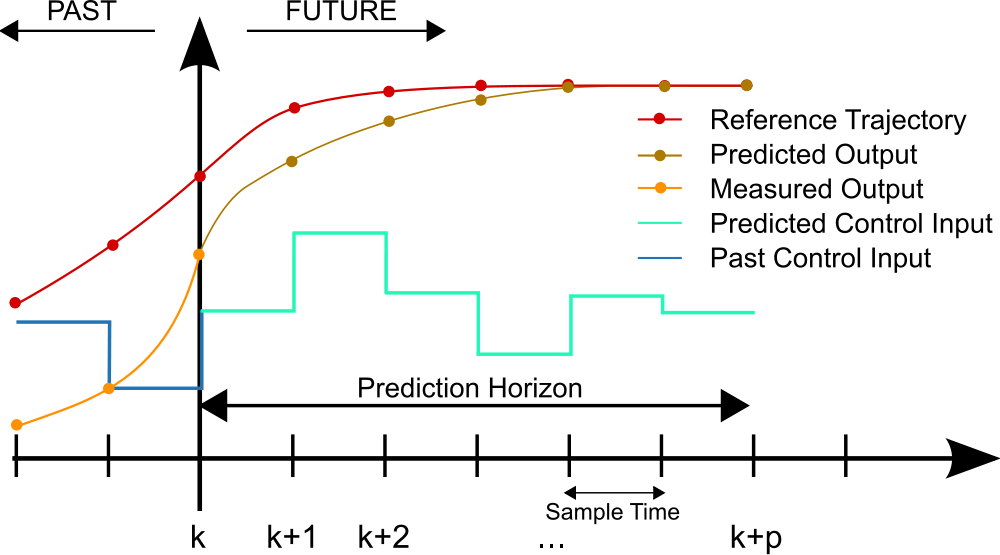
\includegraphics[width=0.85\textwidth,scale=1]{"src/Images/mpc.png"}
	\caption{A simple MPC Scheme \cite{MPC2023}}
	\label{fig:MPC Schematic}
\end{figure}

\clearpage

\subsection{Optimal Control Problems(OCP)}
An optimal control problem involves the mathematical formulation and analysis of determining an optimal trajectory for a dynamic system, subject to constraints and other performance criteria (minimizing the cost function). The OCP for a non-linear system with a quadratic cost function and constraints is as follows: 

\begin{equation}
\underset{\substack{x_0,x_1...x_N \\ u_0,u_1...u_{N-1}}} {\operatorname{min}} \sum_{k=0}^{N-1}\left (x_{k}^{T} Q x_{k}+ u_{k}^{T} R u_{k}\right)+x_{N}^{T} Q_f x_{N}^{T}
\end{equation}

\begin{equation}
\begin{array}{ll}
\text { subject to } & x_{k+1} = f(x_k,u_k)  \\
& x_0 = x(0) \\

& u_k \in \mathbb{U}, x_k \in \mathbb{X} \\

& \forall k \in[0, N-1] \\

& x_N \in \mathbb{X}_f \\
\end{array}
\end{equation}

Where $x_k$ and $u_k$ are the states and inputs respectively of the $k$-th time step and $x_N$ denotes the terminal state.

$Q$ and $R$ matrices are the state and input weight matrices respectively and $Q_f$ is the weight of the terminal state.

 

The constraints include the regular state and input constraints along with the dynamic model of the system as an additional continuity constraint. 

The cost function can be extended to include a different goal state by replacing the $x_k$ term with $(x_k - x_{goal})$.

\subsection{Stability}

While no concrete stability guarantees for Non-Linear MPC (NMPC) can be made, the theory behind Linear MPC has been well established for some time.This can be in practice adapted to NMPC.

The stability analysis of Linear MPC can be divided mainly into two parts :

\textbf{a. Recursive Feasibility}: Since the MPC algorithm involves the solution of an Optimization problem at every time step, one has to ensure that the problem remains feasible. This is done by proper choice of terminal sets. If the terminal set is chosen to be control invariant, one can ensure recursive feasibility. Written down mathematically, if  $\forall x \in \mathbb{X}_f \; \exists \;  \kappa(x) \in \mathbb{U} $ such that  $ f(x, \kappa(x)) \in \mathbb{X}_f $, then one can achieve recursive feasibility \cite{Fang2022, Allgower2004}. 

\textbf{a. Stability of the Origin}: Stability of the MPC algorithm in inherently tied to the choice of the terminal ingredients of the OCP. Recursive feasibility was achieved by selecting a suitable terminal set and likewise the stability at the origin can be confirmed by the right choice of terminal weights. 
A possible choice of terminal set is as follows: 

For positive definite $Q$ and $R$ matrices, solve the infinite horizon LQR problem. Since the infinite horizon LQR results in a constant quadratic optimal cost $P$, this can be assigned as the terminal weight to ensure stability about the origin \cite{Fang2022,Rawlings2017,Allgower2004}.

\subsection{Optimality}

Good choices of terminal ingredients can lead to stability. But sub-optimalities can arise due to the choice of prediction horizon and for any given initial condition there exists a prediction horizon $N_{min}$ that is optimal for the constrained closed loop system.

Any solution that satisfies the constraints is termed to be a feasible solution, whereas the feasible solution with the least cost is called the Optimal solution. 
For any prediction horizon, $N > N_{min}$ the performance of the closed loop does not visibly improve, and if  $N < N_{min}$ and the optimization problem is feasible, the closed loop can still be close to optimality because of the receding horizon (feedback) implementation.
 

  
\clearpage


            \chapter{Development}\label{chap:third chapter}

Since the implementation of the MPC algorithm is on a real system, and optimization is very computationally heavy, performing the computation on the ESP32 microcontroller was not the best way forward. Thus, communication was established between a host PC where all the heavy computation would take place and the microcontroller would be responsible for applying the calculated input and  measuring the states of the pendulum, followed by relaying this information to the host PC. A schematic of this setup can be found in Figure \ref{fig:Comms Schematic}.


\begin{figure}[htbp]
	\centering
	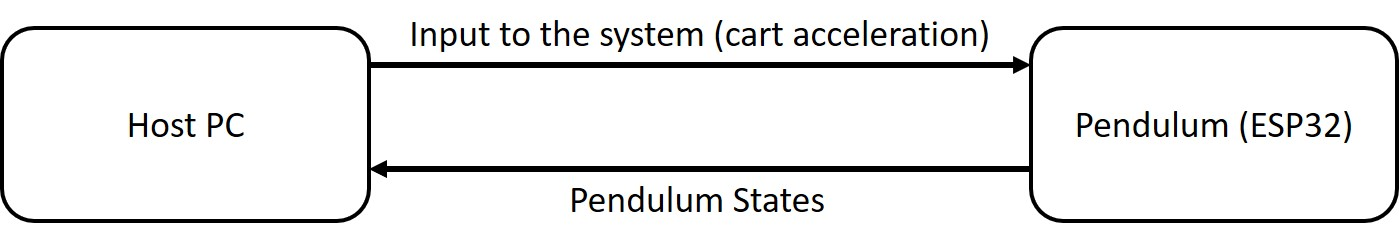
\includegraphics[width=\textwidth]{"src/Images/CommsSchematic.jpg"}   
	\caption{Concept Schematic}
	\label{fig:Comms Schematic}
\end{figure}

In this chapter we will take a look at both halves of this setup with a look into the MPC algorithm on the host PC side, the Arduino interface on the pendulum side and the established communication channel connecting the two halves.

\section{MPC}

As mentioned before, the first half of the system is the host PC where optimization is performed, with Python as the programming language of choice. For the purpose of easy access and understanding we encapsulated the parts into separate classes on python. 2 major tasks are carried out on the PC, namely : optimization and interfacing. In this section we will look at the optimization part in detail, with the interfacing being dealt with in further sections.

\subsection{Optimization on Python} \label{Section 3.1.1}

As suggested in Chapter \ref{Chapter 2}, the optimization problem uses a simple quadratic cost setup. The python script that performs the task of optimization is done with the help of the ACADOS package. ACADOS  is the successor of the ACADO software package developed at KU Leuven and University of Freiburg by the team of Prof. Moritz Diehl \cite{acados}.  

ACADOS offers extremely fast optimization time and makes it possible to run near the real time optimization requirement of the inverted pendulum. 

The state is measured and passed on to the $step()$ function that calculates the next controller step. The algorithm for which is as follows: 


\begin{algorithm}[H]
	\caption{MPC Control step}\label{alg:one}
	\KwData{$x_k$: Data at time step $k$ \\
		\hspace{1.3cm}Solver : a prebuilt ACADOS OCP solver object to be passed as an input to the \\ \hspace{2.5cm}$solve()$ function}
	\KwResult{$u$: Control input for time step $k+1$ }
	
	
	\eIf{first time = "True"}
	{
		initial guess for solver object $\gets$ first initial guess
	}
	%else
	{
		initial guess for solver object $\gets$ warm started initial guess
	}
	
	$x_{opt},u_{opt}$ $\gets$ Solve(solver,initial guess)
	
	$u$ $\gets$ $u_{opt}[0]$ \Comment{First Optimal Input} \\ 
	
	\textbf{Return} : $u$
	
\end{algorithm}

You are free to choose the first initial guess to the solver. Here, we load the solution of the first optimal control problem from a file as the first initial guess. 

As explained before, MPC involves using the first part of the optimal input trajectory to apply on the system. Although the rest of the sequence of inputs is not utilized, it can be reused in the next sampling instant to generate a rough estimate of optimal solution of the next QP problem. This technique is called warm-start and its primary reason is to reduce computational complexity in solving the next QP \cite{Otta2015}.


The optimization strategy used is sequential quadratic programming (SQP). This involves breaking down the problem into smaller quadratic program (QP)subproblems and optimizing each individual quadratic program \cite{Nocedal2006}.

These subproblems are solved using the partial condensing HPIPM(High Performance Interior Point Method). This involves the construction of a barrier function that is used to manage the inequality constraint \cite{Nocedal2006}.

Different solver options were tested and while the regular SQP method was far too slow in calculating the solutions, SQP with real time iterations ($SQP$\_$RTI$) \cite{acados,Diehl2005} was able to compute the solutions extremely fast due to a smaller local horizon . And in the interest of speed, the hessian, which is necessary for the calculation of optimal trajectories, is approximated using the Gauss-Newton approximation. This makes the problem more efficient. 

The optimization problem solved at every iteration is structured like the one described in previous chapters, which is as follows:
\begin{equation}
	\underset{\substack{x_0,x_1...x_N \\ u_0,u_1...u_{N-1}}} {\operatorname{min}} \sum_{k=0}^{N-1}\left (x_{k}^{T} Q x_{k}+ u_{k}^{T} R u_{k}\right)+x_{N}^{T} Q_f x_{N}^{T}
\end{equation}

\begin{equation}
	\begin{array}{ll}
		\text { subject to } & x_{k+1} = f(x_k,u_k)  \\
		& x_0 = x(0) \\
		
		& u_k \in \mathbb{U}, x_k \in \mathbb{X} \\
		
		& \forall k \in[0, N-1] \\
	\end{array}
\end{equation}

The values of $Q_k, R$ and $Q_f$ were tuned for optimal performance. The final values of these parameters are:

\begin{center}
	$Q_k = \begin{bmatrix}
		10 & 0       & 0      & 0      \\                       
		0  & 10^{-4} & 0      & 0      \\
		0  & 0       & 10^{4} & 0      \\
		0  & 0       & 0      & 10^{-2}\\
	\end{bmatrix}
	$
	\hspace{2cm}
	$R = \begin{bmatrix}
		10
	\end{bmatrix}
	$
\end{center}

$Q_f$ is decided by solving the infinite horizon LQR problem with the above mentioned $Q_k$ and $R$ values. This is common practice to achieve stability with MPC.


\section{Pendulum}

The pendulum is operated by the ESP32 microcontroller unit (MCU), a powerful and generic MCU with integrated Wi-Fi and Bluetooth connectivity for a wide range of applications \cite{ESPManual}

Since the ESP32 is an arduino peripheral one can use the arduino IDE to code instructions into the MCU. The ESP main $loop()$ function involves receiving, storing new data using the $recvWithEndMarker()$ and $storeNewData()$ functions. 
The algorithm for the main loop is as follows: 


\begin{algorithm}[H]
	\caption{Pendulum main loop}\label{alg:two}
	\KwData
	{	$x_k$: linear position data at time step k \\
		\hspace{1.4cm}$\theta_k$: angular position data at time step k \\
		\hspace{1.4cm}$dx_k$: linear velocity data at time step k \\
		\hspace{1.4cm}$d\theta_k$: angular velocity data at time step k \\
		\hspace{1.4cm}$u$ : received floating number of the input acceleration
	}
	
	\KwResult{$u_k$: The frequency needed to generate a desired linear velocity corresponding to the input signal.}
	
	
	
	\hspace{2mm}$u \gets read()$  \Comment{read() function reads a byte of serial data and stores it in an array} \\
	
	\hspace{2mm}$\theta_k \gets$ (PendulumEncoderPulses + 800) * 2$\pi$/1600 \\
	$x_k  \gets $ MotorEncoderPulses/20,000  \cite{PendulumManual} \\
	
	\eIf{current time - start time > 5ms}
	{
		$dx_k , d\theta_k \gets $ velocities calculated from measured valued of displacement 
	}
	{
		current time $\gets$ esp\_timer\_get\_time()  \Comment{ This line updates the current time variable}
	}
	
	sendStates($x_k, dx_k, \theta_k, d\theta_k$)      \Comment{Sends the states to the PC every 5ms}
	
	$u_k \gets$ real dynamics() \Comment {}
	
	start time $\gets$ current time    \Comment{This reassigns the start time as the current time}
	
	\textbf{Return} : $u_k$
	
\end{algorithm}
\clearpage


The $real$\_$dynamics()$ function calculates the value of the frequency of the PWM signal needed to generate the required velocity. The values of $x_k$ and $\theta_k$ values from the encoders of the pendulum. 

\begin{eqnarray}
	\theta_k= \frac{PendulumEncoderPulses+800)\cdot 2\pi}{1600} \\
	x_k =  \frac{MotorEncoderPulses}{20,000}
\end{eqnarray}


The encoder generates 400 pulses per revolution per channel. It has two channels, therefore, if the rising and falling edges are encountered, the resulting resolution is 1600 pulses per revolution. If we want to convert the pulses to angle in radians the simple math can be incorporated. And since we want the initial stable equilibrium position to correspond to an angle of $\pi$ radians, we add an additional 800 to the value of the rotary encoder pulses.
Similarly, the position can also be calculated by dividing the motor encoder pulses by a value of 20,000 \cite{PendulumManual}.






\section{Interfacing}

Now that we have established the 2 sides of communication channel, we can elaborate on the channel itself. In this section we will explain in detail the communication procedure on both the PC side and the microcontroller side.


\subsection{PC interface}

As mentioned before, python is the language used for optimization purposes and therefore is used to develop the PC interface of the communication channel as well. pySerial is a popular package for USB communication on Python and that is the package used in this particular application as well.

\textbf{Reading states from microcontroller:}

The Arduino has been programmed to continuously send the pendulum states every 5ms. To trigger the measurement of states on the PC side we use the $measure()$ function.

The read\_all() method in the serial module will read all the data that is available on the serial port and store it in a variable, this forms our buffer. We then extract the last 42 bytes from this buffer. With 4 states, one input and one delimiting character ("?") the total message size is 21 bytes. We extract the most recent 42 bytes in case of incomplete messages. 

The extracted message is then saved 4 bytes at a time to extract the 4 states. 


\textbf{Applying input:}

After calculating the input, $u$, as directed in section \ref{Section 3.1.1}, this input has to be applied to the pendulum cart. This can be done using the $apply()$ function on the PC side. This simply uses the $struct.pack()$ method to convert the input to its binary representation and $pySerial.write()$ function to send it to the pendulum via the connected serial port. 

\subsection{Pendulum interface}

As mentioned before, the pySerial package is used to establish a communication channel between the PC and the ESP32 microcontroller which controls the motor which in turns controls the pendulum. The ESP32 generates pulse width modulated (PWM) signals that cause motion in the stepper motor, generated by the LEDC peripheral on the EPS32, and thereby moving the pendulum cart.  \\


\textbf{Receiving from PC: the read() function}

The read function involves sequentially reading a byte of serial data and storing it in an array until the end of the message. This message is the input to the pendulum. The delimiter for this message is the $'\backslash n'$ symbol. 

\textbf{Sending to PC: real\_dynamics() and sendStates() functions}

The controller's output data is a sequence of four states, each of 4 bytes with the symbol,'?', denoting the start of this sequence.  To decrease the length of the message and increase the communication speed, the recorded floating point data was written as an address using IEEE754 standards instead of sending ASCII data of each number in the message. This is written into the serial buffer by the \textbf{sendStates()} function.

The \textbf{real\_dynamics()} function is responsible for the calculation of the frequency of the PWM signal from the received value of cart acceleration. This can be done using the following relation:

\begin{equation}
	f_{pwm} = v_{cart}\cdot20,000
\end{equation}

This relation comes from the formula for 

While calculating the frequency of the PWM signal, one has to account for the application of both high and low frequency signals. This can be done by adjusting the duty cycle resolution of the ESP32 clock.  Since frequency and duty resolution are inversely related one has to choose a resolution that can handle higher as well as lower frequencies. This can be done using the formula provided in \cite{ESPManual}. 

\begin{eqnarray}
	Duty  =\log_2 \left ( \frac{\mathit{f}_{clock}} {\mathit{f}_{pwm} * N_{clock}} \right)
	\\
	N_{clock} = \mathrm{A} + \frac{\mathrm{B}}{256}
\end{eqnarray}


Here $N_{clock}$ stands for the effective division factor of the arduino clock and the $\mathrm{A,B}$ here stand for the integer and fractional part of the division factor of the divider within the timer.  

From this one can calculate that for high velocities we require a duty resolution of 1-11 bits and for lower velocities we require a duty resolution of 8-20 bits. From this a resolution of 8 bits was chosen. In theory resolutions of 9,10 and 11 bits are also valid choices. 




            \chapter{Results}\label{chap:fourth chapter}

The results of this experiment can be broadly classified into 2 categories, namely simulation results and those of the real system. The following chapter looks into these results in detail.


\section{Simulation Results}

To test the accuracy of the model and the speed of the optimization algorithm, simulations were performed and studied.

For the implementation of the MPC algorithm, the simulation was conducted on the PC, with a simulated pendulum class with internal functions that simulate the behavior of a real pendulum. 

\begin{figure}[H]
	\centering
	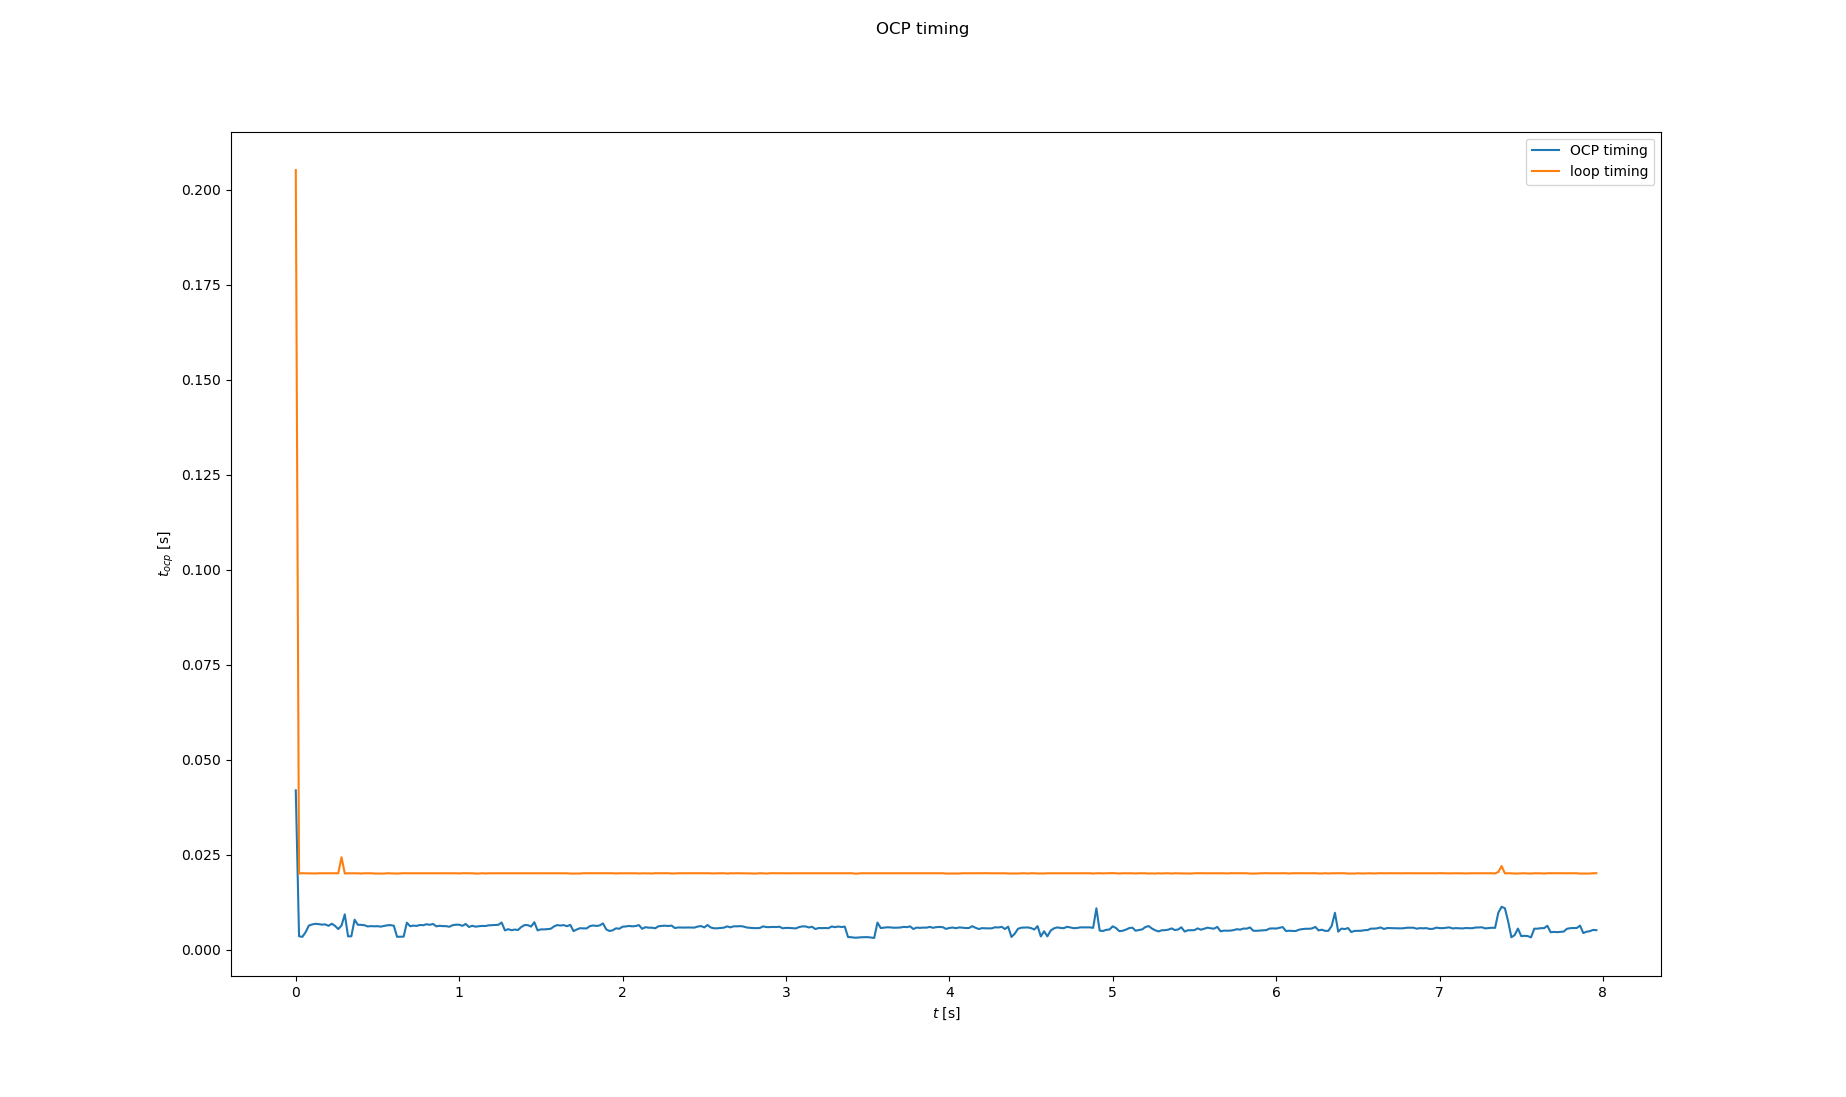
\includegraphics[width=0.96\textwidth]{"src/Images/OCP_Timing_Graph_Pendulum_Simulation.png"}
	\caption{Timing graph: Simulation}
	\label{fig:Timing: Pendulum simulation}
\end{figure}

A necessary condition for proper functioning of the real system is that the measurement of states and the calculation, application of the input must happen within the sampling time of the controller, which is \textbf{20} ms in our case. 

Figure \ref{fig:Timing: Pendulum simulation} depicts the time taken to solve the OCP at every iteration of the main loop and it is solved in less than 10 milliseconds at almost every iteration, which leaves enough time to communicate with the pendulum.


\begin{figure}[H]
	\centering
	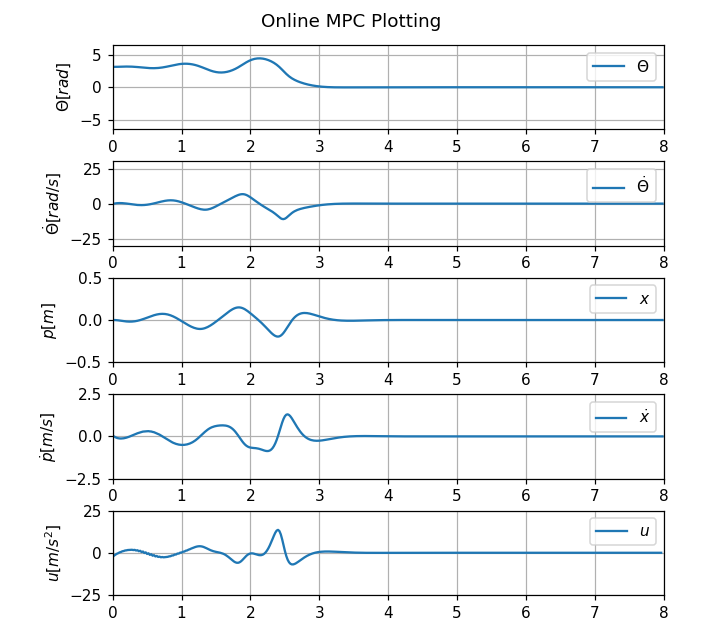
\includegraphics[width=\textwidth]{"src/Images/PC_Simulation_OnlinePlot.png"}
	\caption{Simulation}
	\label{fig:Simulation}
\end{figure}

Figure \ref{fig:Simulation} depicts the states during the MPC algorithm which converges to the origin as is expected.  
 
 \clearpage
 
\section{Real system results}

Upon running the algorithm on the real system, the following results were obtained:

\begin{figure}[H]
	\centering
	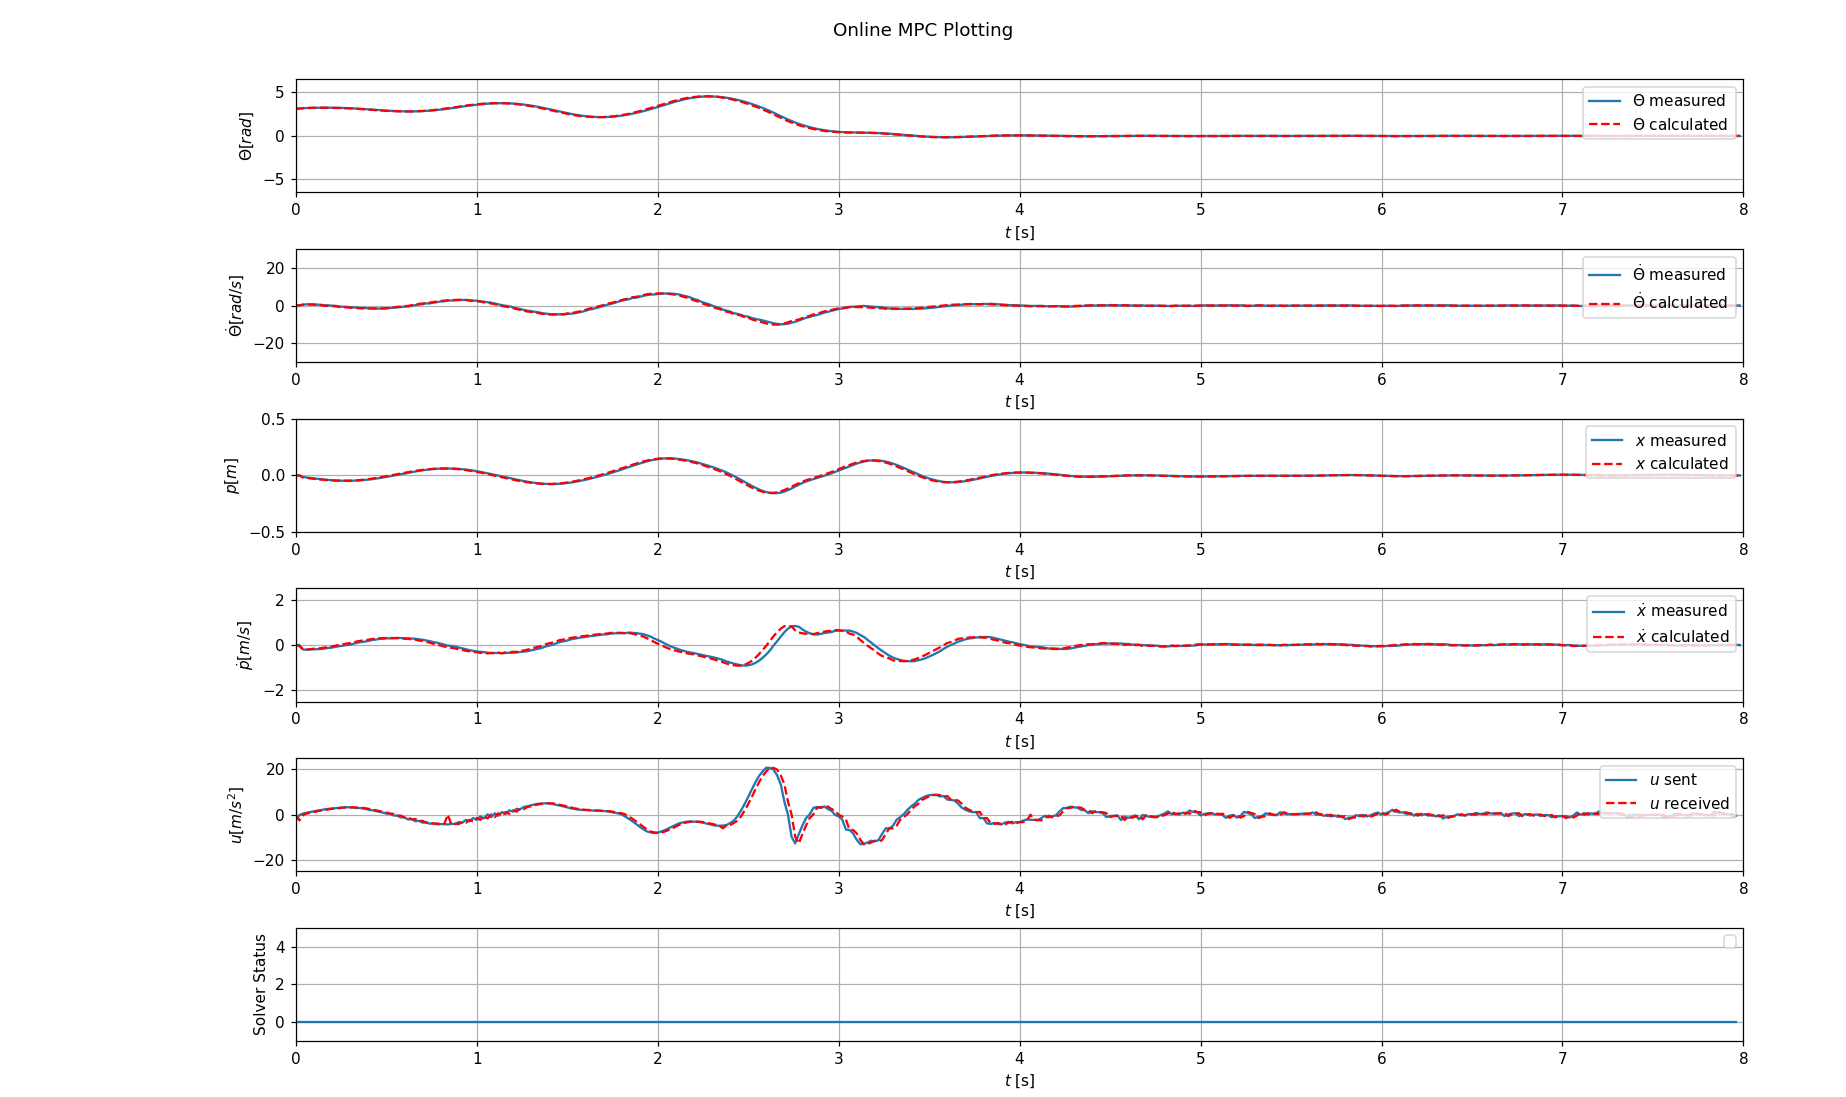
\includegraphics[width=\textwidth]{"src/Images/Real_Pendulum_OnlinePlot.png"}
	\caption{Real Pendulum}
	\label{fig:Real Pendulum Plot}
\end{figure}

As seen here, the states closely converge to the origin and therefore the pendulum stabilizes in an upright position within 3.5-4 seconds. There are also slight disturbances on the input which is expected due to real world factors such as different friction coefficients and drag. 



            \chapter{Conclusion}\label{chap:fifth chapter}

In this chapter we will go over the conclusions drawn from this project and discuss the scope of future projects on this system. 

The complete control system consists of a host PC which is used for computation purposes and an inverted pendulum, produced by Optimal Control Labs, s.r.o. The main aim of this project is to stabilize the pendulum in the upright position at the centre of the rail. This pendulum uses it's in built sensors to measure and/or calculate the states, and is able to provide near perfect state feedback.

Considering the initial requirements, the MPC algorithm does indeed stabilize the pendulum in an upright position. The system responds well to slight disturbances of the pendulum at the unstable equilibrium. Therefore, the requirements of the project have been met successfully. 

\section{Outlook}

The findings suggest that MPC is a promising approach for controlling inverted pendulum systems and other complex and unstable systems. We believe that further work should focus on the following aspects to further enhance the application of MPC in this domain:

\begin{itemize}
	
	\item \textbf{Observer based MPC}: In this project, we were reliant on the system for state feedback, which though mostly accurate, could be improved. State observers like the Kalman filter which reduces the impact of measurement and process noise on the state estimates could be implemented for smoother and more accurate control. 
	
	\item  \textbf{Advanced MPC Algorithms}: Investigating and developing more advanced MPC algorithms can help in improving control performance. Strategies like multi-stage or tube based MPC are promising avenues to look into in this regard.
	
	\item \textbf{Embedded MPC}: As mentioned in Chapter \ref{chap:third chapter} the optimization was performed on the host PC due to the computational complexity of the MPC algorithm. But there is a way to circumvent this. Embedded MPC involves the condensing of the QP and reducing the memory requirement, enough so to perform it on embedded hardware.
	
	\item \textbf{Machine Learning Integration}: Like mentioned before, exploring more complex control algorithms is an encouraging path in moving forward and the next logical step is the integration of machine learning techniques into these control strategies.These methods, like explicit MPC, can lead to less computation heavy control algorithms, which may decrease control complexity and greatly improve overall performance.
	
	
\end{itemize}


In conclusion, MPC offers a powerful and robust control strategy for stabilizing an inverted pendulum system. By further refining the control algorithms, optimizing implementation, and exploring new applications, MPC can continue to play a vital role in addressing challenging control problems in various fields.

		
			
		\backmatter
			\printbibliography
\end{document}